%This work is licensed under the Creative Commons Attribution-ShareAlike 4.0 International License. 
%To view a copy of this license, visit http://creativecommons.org/licenses/by-sa/4.0/ or send a letter 
%  to Creative Commons, PO Box 1866, Mountain View, CA 94042, USA.

\documentclass{jdrp}

\bibliography{chapitres/scenario/DaM-01.references} 

\newcommand*{\crg}{{\aurebesh\Large \$}} % Symbol for Galactic Credits

\hypersetup{
	pdftitle={SWR - Dos au Muur},
	pdfsubject={Scénario, Dos au Muur},
	pdfauthor={Marthym},
	pdfkeywords={starwars,savage,worlds,jdr,scenario},
	pdfcopiright={This work is licensed under the Creative Commons Attribution-ShareAlike 4.0 International License.}
}

\begin{document}

	\begin{titlepage}
		Dos au Muur

		Sauvetage du Pelican
	\end{titlepage}

Voici un scénario d'introduction pour la campagne \textbf{Dos au Muur}. Cette campagne est écrite initialement pour \citetitle{jdrp-starwars} mais un scénar reste un scénar et il est jouable dans n'importe quel univers de Star Wars.

Il est adaptable aussi bien avec des joueurs orienté Alliance Rebelle que Empire. Dans les deux cas, l'objectif sera le même mais les dessains changeront.

La campagne est faite pour des joueurs débutant, partant du rang Novice.

\section{contexte de campagne}
La campagne se déroule dans les premières années de l'avènement de l'Empire, au MJ de voir s'il veut préciser.

L'objectif de la campagne est de retrouver un très ancien artéfact, le \textbf{Talisman de Muur}. Un artéfact créé par Karness Muur, un Sith se servant de la Force pour prolonger sa vie. L'artéfact contient l'âme de Muur, celui qui le porte est possédé par Karness et peut contrôller les Rakghoules.

Mais nous verrons plus en détails au cours de la quête.

\vspace{-1\baselineskip}
\hspace{-0.4\columnsep}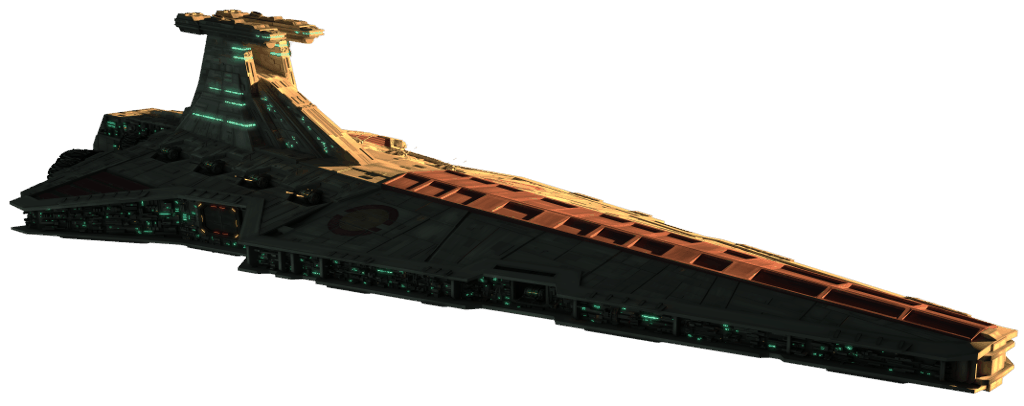
\includegraphics[width=\textwidth]{img/scenario/venator.png}
\vspace{-7\baselineskip}

\section{Sauvetage du Pelican}
\subsection{La rencontre}
Nos héros ne se connaisent pas encore. Ils ont répondu à un contract proposé par \emph{Industrial Automaton} pour une mission de récupération.

Ils ont rendez-vous sur l'avant poste commercial de l'anneau de Kafrene au Starlord Café. \'A leur arrivé, ils sont conviés dans une arrière salle ou les attend Vyna Anen un Sluissi, le représentant de IA. En plus du groupe de nos héros, deux autres personnes ont répondu au contract, un Abyssin et un Rodien.

\begin{quote}
	Messieurs bonjour, je représente Indrustrial Automaton.
	Comme vous avez peu le voir sur le contract auquel vous avez répondu, nous cherchons a rassembler une équipe pour récupérer l'un de nos prototype de droïde Type R perdu sur Croiseur dont nous n'avons plus de nouvelle.
	Le \textbf{Pelican IA-1701} n'a plus donné signe de vie depuis 10h et 33mn maintenant. Il avait a son bord le seul prototype de notre dernier Type R. Il est vital pour nous de récupérer ce prototype intact.

	Si vous acceptez la mission, une navette droïde vous conduira directement à la dernière position connu du Pelican. Cette mission doit resté confidentielle, nous ne tenons pas à ce que le public sache qu'Industrial Automaton perde ses vaisseau !
	En cas de succés la somme convenue sera virée directement sur vos comptes respectif. Dans le cas contraire vous serez mort ou en passe de l'être.

	Il y a t'il des questions ?

	\ldots

	Bien, la navette décollera de l'astroport, quai N°5 dans une heure, elle n'attendra personne.
\end{quote}

Voilà qui donne le ton et la direction du scénario. Les héros disposent donc d'une heure, s'ils le souhaitent pour faire quelques amplettes puis direction la navette.

\subsection{Pelican Baie}
\begin{flushright} 
	\begin{minipage}[r]{0.7\linewidth}
		\hspace{-2\baselineskip}\'A la sortie d'hyperespace, les héros trouvent croiseur de classe Venator en bon état mais à la dérive.
	\end{minipage}
\end{flushright} 

\begin{flushright}
	\emph{Pelican (IA-1701)}
\end{flushright}

\vspace{5\baselineskip}
La navette tente une procédure d'appomtage mais le système de guidage ne semble pas fonctionner, le droïde aux commande de la navette ne cesse de répéter 

\begin{quote}
	Erreur trop bas tros bas !\\
	Erreur trop bas tros bas !\\
	Erreur trop bas tros bas !\\
	Erreur trop bas tros bas !\\
	\ldots
\end{quote}

Et la navette s'échoue lamentablement dans le hangard. Comme de par hasard, et pour bien appuyer sur le gravité de la situation, l'Abyssin et le Rodien sont mort pendant le crash et le droïde pilote est dans un sale état. Il ne pourra donner aucune information.

Une fois à bord du Pelican, une alarme est en cours et une voie pré-enregistré se fait entendre à intervale régulier :

\begin{quote}
	Alerte trajectoire, un corps celeste croisera la trajectoire actuelle du vaisseau dans 2h53mn ! Voyez modifier la trajactoire du vaisseau !
	\ldots
\end{quote}

\'A l'intérieur du vaisseau c'est la désolation, des cadavres partout, du sang sur les murs, des traces de griffures sur les murs. L'éclairage est partiellement en panne les neons scintilles, des débrits entravent la marche des héros. Leur champ de vision est réduit à cause des conditions à bord. Malgrés tout ça, les systèmes de survit et la gravité artificielle fonctionne.

Le but des héros devrait maintenant être double, trouver le fameux prototype mais aussi trouver un moyen de dévier le vaisseau.


---


Une fois sur place, le vaisseau, un destroyer de classe stellaire est dans un sale état et l'alarme a l'interieur est allumé. Il faut l'arréter grace a un panneau clignotant sur le coté. Une fois l'alarme arrété, la voie d'un robot se faire entendre via les haut parleurs du vaisseau leur expliquant qu'ils ont bien stopé l'alarme mais que le système d'auto-destruction est en court et qu'il ne leure reste que 2h (la durée du scénar) pour rebooter le système.

Ils doivent donc chercher la salle de controle mais ils croisent des ennemis pour se défouler un peu. On commence à comprendre pourquoi le vaisseau est échoué.

Arrivé dans la salle de controle, un droide de compagnie est là, leur explique comment rebouté et leur fais part d'un message expliquant un peu la situation. C'est un message holo où l'on voit un pilote de l'alliance rebelle qui demande à qui trouvera le message de prévenir les rebelles. Un ancien temple Jedi a été retrouvé, et avec lui un ancien artéfact, l'empire ne doit pas mettre la main dessus.

Ils arrivent ou non à rebooter les systèmes dans tous les cas, s'ils y parviennent cela n'arrète pas le compte à rebour. Mais le droide leur dit qu'il reste peut être dans la soute un vaisseau en état de fonctionnement. L'idée est de leur donner ce vaisseau pour qu'ils puissent s'enfuir et faire le reste de la campagne avec.

C'est là que les joueurs doivent choisir leur orientation, Aliance ou Empire. Selon leur choix, soit il partent à l'alliance soit ils partent voir l'empire. Dans tout les cas, ils ont les coordonnées d'un lieu de rendez vous ou un messagé de l'alliance les attends.

http://www.starwars-holonet.com/encyclopedie/technologie-talisman-muur.html

	\onecolumn
	\nocite{*}
	\printbibliography
\end{document}


